\section{Signale}
\label{sec:signale}

\begin{frame}{Verteilung der zivilen Frequenzen}
    \begin{table}
        \begin{tabular}{c l}
            \toprule
            {Satellit} & {Frequenzen} \\
            \midrule
            Block IIA   & L1 C/A \\
            Block IIR   & L1 C/A, L1 P(Y) \\
            Block IIR-M & L1 C/A, L1 P(Y), L2C \\
            Block IIF   & L1 C/A, L1 P(Y), L2C, L5 \\
            GPS III     & L1 C/A, L1 P(Y), L2C, L5, L1C \\
            GPS IIIF    & L1 C/A, L1 P(Y), L2C, L5, L1C \\
            \bottomrule
        \end{tabular}
    \end{table}
\end{frame}

\begin{frame}{Das Signal}
    \begin{columns}
        \begin{column}{0.5\textwidth}
            Informationen im Signal
            \begin{itemize}
                \item Satellitenposition
                \item Zeit
                \item Uhrzeitkorrekturen
                \item Systeminformationen
                \end{itemize}\pause
        \end{column}
        \begin{column}{0.5\textwidth}
            \begin{figure}
                \centering
                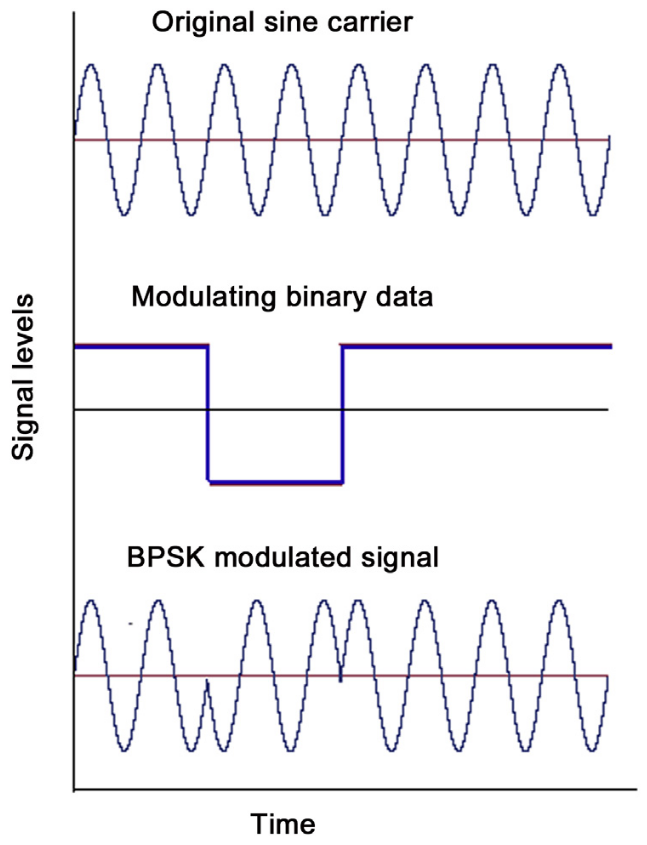
\includegraphics[width=0.5\textwidth]{images/signalzusammensetzung.png}
            \end{figure}
            Wellenzusammensetzung {\small[Acharya]}
        \end{column}
    \end{columns}
\end{frame}
